\documentclass[10pt]{article}

\usepackage{graphicx}
\usepackage{epstopdf}
\usepackage{float}
\usepackage[T1]{fontenc}
\usepackage[titletoc]{appendix}
\usepackage[margin=0.7in]{geometry}
\usepackage{blindtext}
\usepackage[english]{babel}
\usepackage{multirow}
\usepackage{courier}
\usepackage{fancyhdr}
\usepackage{makecell}
\usepackage{caption}
\usepackage{rotating}
\usepackage{pdflscape}
\pagestyle{fancy}
\lhead{Tim Yao - ty252}

\renewcommand{\thesubsection}{\thesection.\alph{subsection}}

\usepackage{listings}
\usepackage{color}

\definecolor{dkgreen}{rgb}{0,0.6,0}
\definecolor{gray}{rgb}{0.5,0.5,0.5}
\definecolor{mauve}{rgb}{0.58,0,0.82}

\lstset{frame=tb,
  language=Verilog,
  aboveskip=3mm,
  belowskip=3mm,
  showstringspaces=false,
  columns=flexible,
  keepspaces=true,
  numbers=left,
  basicstyle={\small\ttfamily},
  keywordstyle=\color{blue},
  commentstyle=\color{dkgreen},
  stringstyle=\color{mauve},
  breaklines=false,
  breakatwhitespace=true,
  tabsize=2
}

% For monospace stuff

\title{ECE 4750 PSET 4}
\author{Tim Yao (ty252)}
\date{Nov 25, 2015}

\begin{document}
\maketitle
\newcommand*{\tableindent}{\hspace*{0.3cm}}%
Worked with Gautam Ramaswamy, Gaurab Bhattacharya, and Sacheth Hegde.
\section{Tree Network Topologies} 

\subsection{Baseline I3L Microarchitecture}
\begin{figure}[H]
\centering
{\setlength{\tabcolsep}{2pt}
\begin{tabular}{|l|c|c!{\vrule width 1.5pt}c|c|c|c|c|c|c|c|c|c|c|c|c|c|c|c|c|c|c|c|c|c|c|c|c|c|c!{\vrule width 1.5pt}}
\hline
Cycle:            & 0 & 1 & 2 & 3 & 4 & 5 & 6 & 7 & 8 & 9 & 10 & 11 & 12 & 13 & 14 & 15 & 16 & 17 & 18 & 19 & 20 & 21 & 22 & 23 & 24 & 25 & 26 & 27 & 28 \\ \hline
mul r1, r2, r3    & F & D & I & Y0& Y1& Y2& Y3& W &   &   &    &    &    &    &    &    &    &    &    &    &    &    &    &    &    &    &    &    &    \\ \hline
mul r4, r1, r5    &   & F & D & I & I & I & I & Y0& Y1& Y2& Y3 & W  &    &    &    &    &    &    &    &    &    &    &    &    &    &    &    &    &    \\ \hline
div r6, r7, r8    &   &   & F & D & D & D & D & I & Z & Z & Z  & Z  & W  &    &    &    &    &    &    &    &    &    &    &    &    &    &    &    &    \\ \hline
div r9, r10, r11  &   &   &   & F & F & F & F & D & I & I & I  & I  & Z  & Z  & Z  & Z  & W  &    &    &    &    &    &    &    &    &    &    &    &    \\ \hline
div r12, r13, r14 &   &   &   &   &   &   &   & F & D & D & D  & D  & I  & I  & I  & I  & Z  & Z  & Z  & Z  & W  &    &    &    &    &    &    &    &    \\ \hline
mul r15, r12, r16 &   &   &   &   &   &   &   &   & F & F & F  & F  & D  & D  & D  & D  & I  & I  & I  & I  & Y0 & Y1 & Y2 & Y3 & W  &    &    &    &    \\ \hline
mul r17, r15, r18 &   &   &   &   &   &   &   &   &   &   &    &    & F  & F  & F  & F  & D  & D  & D  & D  & I  & I  & I  & I  & Y0 & Y1 & Y2 & Y3 & W  \\ \hline
\end{tabular}
}
\caption{Pipeline Diagram for Baseline I3L Architecture}
\end{figure}

The total issue to commit cycle count is 27.

\subsection{Schedule Oldest Ready Instruction First on IO2L Microarchitecture}

\begin{figure}[H]
\centering
{\setlength{\tabcolsep}{2pt}
\begin{tabular}{|l!{\vrule width 1.5pt}c|c|c|c|c|c|c|c|c|c|c|c|c|c|c|c|c|c|c|c|c|c|c|c!{\vrule width 1.5pt}}
\hline
Cycle:            & 0 & 1 & 2 & 3 & 4 & 5 & 6 & 7 & 8 & 9 & 10 & 11 & 12 & 13 & 14 & 15 & 16 & 17 & 18 & 19 & 20 & 21 & 22 & 23 \\ \hline
mul r1, r2, r3    & I & Y0& Y1& Y2& Y3& W & C &   &   &   &    &    &    &    &    &    &    &    &    &    &    &    &    &    \\ \hline
mul r4, r1, r5    &   &   &   &   & I & Y0& Y1& Y2& Y3& W & C  &    &    &    &    &    &    &    &    &    &    &    &    &    \\ \hline
div r6, r7, r8    &   & I & Z & Z & Z & Z & W & r & r & r & r  & C  &    &    &    &    &    &    &    &    &    &    &    &    \\ \hline
div r9, r10, r11  &   &   &   &   &   & I & Z & Z & Z & Z & W  & r  & C  &    &    &    &    &    &    &    &    &    &    &    \\ \hline
div r12, r13, r14 &   &   &   &   &   &   &   &   &   & I & Z  & Z  & Z  & Z  & W  & C  &    &    &    &    &    &    &    &    \\ \hline
mul r15, r12, r16 &   &   &   &   &   &   &   &   &   &   &    &    &    & I  & Y0 & Y1 & Y2 & Y3 & W  & C  &    &    &    &    \\ \hline
mul r17, r15, r18 &   &   &   &   &   &   &   &   &   &   &    &    &    &    &    &    &    & I  & Y0 & Y1 & Y2 & Y3 & W  & C  \\ \hline
\end{tabular}
}
\caption{Pipeline Diagram for IO2L Architecture}
\end{figure}

The total issue to commit cycle count is 24.

\subsection{Optimal Scheduling on IO2L Microarchitecture}

\begin{figure}[H]
\centering
{\setlength{\tabcolsep}{2pt}
\begin{tabular}{|l!{\vrule width 1.5pt}c|c|c|c|c|c|c|c|c|c|c|c|c|c|c|c!{\vrule width 1.5pt}}
\hline
Cycle:            & 0 & 1 & 2 & 3 & 4 & 5 & 6 & 7 & 8 & 9 & 10 & 11 & 12 & 13 & 14 & 15 \\ \hline
div r12, r13, r14 & I & Z & Z & Z & Z & W & C &   &   &   &    &    &    &    &    &    \\ \hline
mul r1, r2, r3    &   & I & Y0& Y1& Y2& Y3& W & C &   &   &    &    &    &    &    &    \\ \hline
div r6, r7, r8    &   &   &   &   & I & Z & Z & Z & Z & W & C  &    &    &    &    &    \\ \hline
mul r15, r12, r16 &   &   &   &   &   & I & Y0& Y1& Y2& Y3& W  & C  &    &    &    &    \\ \hline
mul r4, r1, r5    &   &   &   &   &   &   & I & Y0& Y1& Y2& Y3 & W  & C  &    &    &    \\ \hline
div r9, r10, r11  &   &   &   &   &   &   &   &   & I & Z & Z  & Z  & Z  & W  & C  &    \\ \hline
mul r17, r15, r18 &   &   &   &   &   &   &   &   &   & I & Y0 & Y1 & Y2 & Y3 & W  & C  \\ \hline
\end{tabular}
}
\caption{Pipeline Diagram for IO2L Architecture}
\end{figure}

The total issue to commit cycle count is 16.

\subsection{Scheduling Comparison}

TODO!

\cleardoublepage
\section{Register Renaming}

\subsection{Architectural RAW, WAW, and WAR Dependencies}

\begin{lstlisting}
mul  r1, r2, r3
mul  r4, r1, r5
addu r6, r7, r8
mul  r1, r2, r5
addu r6, r6, r9
\end{lstlisting}

\subsection{Pipeline Diagram with Register Renaming}

\begin{figure}[H]
\centering
{\setlength{\tabcolsep}{2pt}
\begin{tabular}{|l|c|c|c|c|c|c|c|c|c!{\vrule width 1.5pt}c!{\vrule width 1.5pt}c!{\vrule width 1.5pt}c!{\vrule width 1.5pt}c|}
\hline
Cycle:            & 0 & 1 & 2 & 3 & 4 & 5 & 6 & 7 & 8 & 9 & 10 & 11 & 12 & 13 & 14 & 15 \\ \hline
mul  r1, r2, r3   & F & D & I & Y0& Y1& Y2& Y3& W & C &   &    &    &    &    &    &    \\ \hline
mul  r4, r1, r5   &   & F & D & i & i & i & I & Y0& Y1& Y2& Y3 & W  & C  &    &    &    \\ \hline
addu r6, r7, r8   &   &   & F & D & I & X & W & r & r & r & r  & r  & r  & C  &    &    \\ \hline
mul  r1, r2, r5   &   &   &   & F & D & I & Y0& Y1& Y2& Y3& W  & r  & r  & r  & C  &    \\ \hline
addu r6, r6, r9   &   &   &   &   & F & D & i & I & X & W & r  & r  & r  & r  & r  & C  \\ \hline
\end{tabular}
}
\caption{Pipeline Diagram for Elastic Buffering with Two-Element Channel Buffers}
\end{figure}
As show by the bolded vertical lines, in steady state, it takes 1 cycle to move a packet. This gives a peak terminal throughput of 1 packet per cycle.\\
The ideal flow control should provide 1 packet per cycle. This design is able to achieve the throughput of ideal flow control.

\subsection{Pipeline Diagram for Round-Robin Arbitration}

\begin{figure}[H]
\centering
{\setlength{\tabcolsep}{2pt}
\begin{tabular}{|l|c|c|c|c|c|c|c|c|c|c|c|c|c|}
\hline
Cycle: & 1  & 2  & 3  & 4  & 5  & 6  & 7  & 8  & 9  & 10 & 11 & 12 & 13 \\ \hline
pkt0-2 & I  & R0 & L0 & L1 & R1 & O  &    &    &    &    &    &    &    \\ \hline
pkt0-3 & I  & R0 & R0 & L0 & L1 & R1 & O  &    &    &    &    &    &    \\ \hline
pkt1-2 &    & I  & R0 & R0 & L0 & L1 & R1 & O  &    &    &    &    &    \\ \hline
pkt1-3 &    & I  & q  & R0 & R0 & L0 & L1 & R1 & O  &    &    &    &    \\ \hline
pkt2-2 &    &    & I  & q  & R0 & R0 & L0 & L1 & R1 & O  &    &    &    \\ \hline
pkt2-3 &    &    & I  & q  & q  & R0 & R0 & L0 & L1 & R1 & O  &    &    \\ \hline
pkt3-2 &    &    &    & I  & q  & q  & R0 & R0 & L0 & L1 & R1 & O  &    \\ \hline
pkt3-3 &    &    &    & I  & q  & q  & q  & R0 & R0 & L0 & L1 & R1 & O  \\ \hline
\end{tabular}
}
\caption{Pipeline Diagram for Round-Robin Arbitration}
\end{figure}
There is no steady state. As shown by the pipeline diagram, the number of elements in the $R_{0,1}$ queue continues to increase. This is due to the the $C_{0,3}$ channel not able to sustain the required throughput (2 phits per cycle). This means that packets will need to be stalled in R0 during arbitration and therefore cause future packets to be continuously queued up. 

\subsection{Global Fairness for Round-Robin Arbitration}
No, the network does not have global strong fairness.\\
Assume that initially, the priority goes to the top input port. In our traffic pattern, inputs 0, 1, and 2 will try to send their packets to output 1, and input 3 will try to send its packets to output 3. First, we see that both inputs 0 and 1 try to access channel $C_{0,0}$, so round-robin arbitration will occur. This means on channel $C_{0,0}$, inputs 0 and 1 will each receive 50$\%$ of the bandwidth. In $R_{0,1}$, because input 2 will access the top output to channel $C_{0,2}$ and input 3 will access the bottom output to channel $C_{0,3}$. Therefore, no arbitration is needed and each channel can sustain full bandwidth from a single input. In $R_{1,1}$, the bottom input coming from channel $C_{0,3}$ will always go to output 3, so again, no arbitration is needed. This means that the requests from input 3 will always be served. In $R_{1,0}$, both inputs want to access output 1, so arbitration is needed. This means that 50$\%$ of the bandwidth comes from the top input (coming from channel $C_{0,0}$) and the other 50 comes from the bottom input (from channel $C_{0,2}$). This means that on output 1, 50$\%$ of the bandwidth comes from input 2, 25$\%$ from input 1, and 25$\%$ from input 0. From this we can see that requests from all inputs are NOT served equally often. 
\cleardoublepage
\section{In-Order Superscalar Processors}

\subsection{Pipeline Diagram for Single-Issue PARCv1 Processor}

\begin{figure}[H]
\centering
{\setlength{\tabcolsep}{2pt}
\begin{tabular}{|l|c|c|c|c!{\vrule width 1.5pt}c|c|c|c|c|c|c|c|c|c|c|c!{\vrule width 1.5pt}c|c|}
\hline
Cycle:            & 1 & 2 & 3 & 4 & 5 & 6 & 7 & 8 & 9 & 10 & 11 & 12 & 13 & 14 & 15 & 16 & 17 & 18 \\ \hline
lw r1 , 0(r2)     & F & D & X & M & W &   &   &   &   &    &    &    &    &    &    &    &    &    \\ \hline
lw r3 , 0(r4)     &   & F & D & X & M & W &   &   &   &    &    &    &    &    &    &    &    &    \\ \hline
mul r1, r1, r6    &   &   & F & D & X & M & W &   &   &    &    &    &    &    &    &    &    &    \\ \hline
mul r3, r3, r7    &   &   &   & F & D & X & M & W &   &    &    &    &    &    &    &    &    &    \\ \hline
addu r8, r1, r3   &   &   &   &   & F & D & X & M & W &    &    &    &    &    &    &    &    &    \\ \hline
addu r9, r9, r8   &   &   &   &   &   & F & D & X & M & W  &    &    &    &    &    &    &    &    \\ \hline
addiu r2, r2, 4   &   &   &   &   &   &   & F & D & X & M  & W  &    &    &    &    &    &    &    \\ \hline
addiu r4, r4, 4   &   &   &   &   &   &   &   & F & D & X  & M  & W  &    &    &    &    &    &    \\ \hline
addiu r10, r10, -1&   &   &   &   &   &   &   &   & F & D  & X  & M  & W  &    &    &    &    &    \\ \hline
bne r10, r0, loop &   &   &   &   &   &   &   &   &   & F  & D  & X  & M  & W  &    &    &    &    \\ \hline
opA               &   &   &   &   &   &   &   &   &   &    & F  & D  & -  & -  & -  &    &    &    \\ \hline
opB               &   &   &   &   &   &   &   &   &   &    &    & F  & -  & -  & -  & -  &    &    \\ \hline
lw r1 , 0(r2)     &   &   &   &   &   &   &   &   &   &    &    &    & F  & D  & X  & M  & W  &    \\ \hline
lw r3 , 0(r4)     &   &   &   &   &   &   &   &   &   &    &    &    &    & F  & D  & X  & M  & W  \\ \hline
\end{tabular}
}
\caption{Pipeline Diagram for Single-Issue PARCv1 Processor}
\end{figure}
As shown by the bold vertical lines, each loop takes 12 cycles to execute. The CPI is therefore 12/10 = 1.2. The IPC is 1/CPI = 0.833.\\
CPI = 1.2 cycles/instruction\\
IPC = 0.83 instructions/cycle\\

\subsection{Pipeline Diagram for Dual-Issue PARCv1 Processor}

\begin{figure}[H]
\centering
{\setlength{\tabcolsep}{2pt}
\begin{tabular}{|l|c|c|c|c!{\vrule width 1.5pt}c|c|c|c|c|c|c|c|c|c|c!{\vrule width 1.5pt}c|c|}
\hline
Cycle:            & 1  & 2  & 3  & 4  & 5  & 6  & 7  & 8  & 9  & 10 & 11 & 12 & 13 & 14 & 15 & 16 & 17 \\ \hline
lw r1 , 0(r2)     & F  & D  & B0 & B1 & W  &    &    &    &    &    &    &    &    &    &    &    &    \\ \hline
lw r3 , 0(r4)     & F  & D  & D  & B0 & B1 & W  &    &    &    &    &    &    &    &    &    &    &    \\ \hline
mul r1, r1, r6    &    & F  & F  & D  & A0 & A1 & W  &    &    &    &    &    &    &    &    &    &    \\ \hline
mul r3, r3, r7    &    & F  & F  & D  & D  & A0 & A1 & W  &    &    &    &    &    &    &    &    &    \\ \hline
addu r8, r1, r3   &    &    &    & F  & F  & D  & A0 & A1 & W  &    &    &    &    &    &    &    &    \\ \hline
addu r9, r9, r8   &    &    &    & F  & F  & D  & D  & B0 & B1 & W  &    &    &    &    &    &    &    \\ \hline
addiu r2, r2, 4   &    &    &    &    &    & F  & F  & D  & A0 & A1 & W  &    &    &    &    &    &    \\ \hline
addiu r4, r4, 4   &    &    &    &    &    & F  & F  & D  & B0 & B1 & W  &    &    &    &    &    &    \\ \hline
addiu r10, r10, -1&    &    &    &    &    &    &    & F  & D  & B0 & B1 & W  &    &    &    &    &    \\ \hline
bne r10, r0, loop &    &    &    &    &    &    &    & F  & D  & D  & A0 & A1 & W  &    &    &    &    \\ \hline
opA               &    &    &    &    &    &    &    &    & F  & F  & D  & -  & -  & -  &    &    &    \\ \hline
opB               &    &    &    &    &    &    &    &    & F  & F  & D  & -  & -  & -  &    &    &    \\ \hline
opC               &    &    &    &    &    &    &    &    &    &    & F  & -  & -  & -  & -  &    &    \\ \hline
opD               &    &    &    &    &    &    &    &    &    &    & F  & -  & -  & -  & -  &    &    \\ \hline
lw r1 , 0(r2)     &    &    &    &    &    &    &    &    &    &    &    & F  & D  & B0 & B1 & W  &    \\ \hline
lw r3 , 0(r4)     &    &    &    &    &    &    &    &    &    &    &    & F  & D  & D  & B0 & B1 & W  \\ \hline
\end{tabular}
}
\caption{Pipeline Diagram for Dual-Issue PARCv1 Processor}
\end{figure}
As shown by the bold vertical lines, each loop takes 11 cycles to execute. The CPI is therefore 11/10 = 1.1. The IPC is 1/CPI = 0.910.\\
CPI = 1.1 cycles/instruction\\
IPC = 0.91 instructions/cycle\\

\subsection{Optimized Pipeline Diagram for Dual-Issue PARCv1 Processor}

\begin{lstlisting}
lw r1 , 0(r2)     
addiu r2, r2, 4   
lw r3 , 0(r4)     
addiu r4, r4, 4   
mul r1, r1, r6    
addiu r10, r10, -1
mul r3, r3, r7    
addu r8, r1, r3   
addu r9, r9, r8   
bne r10, r0, loop                
\end{lstlisting}

\begin{figure}[H]
\centering
{\setlength{\tabcolsep}{2pt}
\begin{tabular}{|l|c|c|c|c!{\vrule width 1.5pt}c|c|c|c|c|c|c|c!{\vrule width 1.5pt}c|}
\hline
Cycle:            & 1  & 2  & 3  & 4  & 5  & 6  & 7  & 8  & 9  & 10 & 11 & 12 & 13 \\ \hline
lw r1 , 0(r2)     & F  & D  & B0 & B1 & W  &    &    &    &    &    &    &    &    \\ \hline
addiu r2, r2, 4   & F  & D  & A0 & A1 & W  &    &    &    &    &    &    &    &    \\ \hline
lw r3 , 0(r4)     &    & F  & D  & B0 & B1 & W  &    &    &    &    &    &    &    \\ \hline
addiu r4, r4, 4   &    & F  & D  & A0 & A1 & W  &    &    &    &    &    &    &    \\ \hline
mul r1, r1, r6    &    &    & F  & D  & A0 & A1 & W  &    &    &    &    &    &    \\ \hline
addiu r10, r10, -1&    &    & F  & D  & B0 & B1 & W  &    &    &    &    &    &    \\ \hline
mul r3, r3, r7    &    &    &    & F  & D  & A0 & A1 & W  &    &    &    &    &    \\ \hline
addu r8, r1, r3   &    &    &    & F  & D  & D  & B0 & B1 & W  &    &    &    &    \\ \hline
addu r9, r9, r8   &    &    &    &    & F  & F  & D  & B0 & B1 & W  &    &    &    \\ \hline
bne r10, r0, loop &    &    &    &    & F  & F  & D  & A0 & A1 & W  &    &    &    \\ \hline
opA               &    &    &    &    &    &    & F  & D  & -  & -  & -  &    &    \\ \hline
opB               &    &    &    &    &    &    & F  & D  & -  & -  & -  &    &    \\ \hline
opC               &    &    &    &    &    &    &    & F  & -  & -  & -  & -  &    \\ \hline
opD               &    &    &    &    &    &    &    & F  & -  & -  & -  & -  &    \\ \hline
lw r1 , 0(r2)     &    &    &    &    &    &    &    &    & F  & D  & B0 & B1 & W  \\ \hline
addiu r2, r2, 4   &    &    &    &    &    &    &    &    & F  & D  & A0 & A1 & W  \\ \hline
\end{tabular}
}
\caption{Optimized Pipeline Diagram for Dual-Issue PARCv1 Processor}
\end{figure}

As shown by the bold vertical lines, each loop takes 8 cycles to execute. The CPI is therefore 8/10 = 0.8. The IPC is 1/CPI = 1.25.\\
CPI = 0.8 cycles/instruction\\
IPC = 1.25 instructions/cycle

\subsection{Optimized Pipeline Diagram for Quad-Issue PARCv1 Processor}

\begin{lstlisting}
lw r1 , 0(r2)     
addiu r2, r2, 4   
lw r3 , 0(r4)     
addiu r4, r4, 4   
mul r1, r1, r6    
addiu r10, r10, -1
mul r3, r3, r7    
addu r8, r1, r3   
addu r9, r9, r8   
bne r10, r0, loop                
\end{lstlisting}

\begin{figure}[H]
\centering
{\setlength{\tabcolsep}{2pt}
\begin{tabular}{|l|c|c|c|c!{\vrule width 1.5pt}c|c|c|c|c|c|c!{\vrule width 1.5pt}c|}
\hline
Cycle:            & 1  & 2  & 3  & 4  & 5  & 6  & 7  & 8  & 9  & 10 & 11 & 12 \\ \hline
lw r1 , 0(r2)     & F  & D  & B0 & B1 & W  &    &    &    &    &    &    &    \\ \hline
addiu r2, r2, 4   & F  & D  & A0 & A1 & W  &    &    &    &    &    &    &    \\ \hline
lw r3 , 0(r4)     & F  & D  & H0 & H1 & W  &    &    &    &    &    &    &    \\ \hline
addiu r4, r4, 4   & F  & D  & G0 & G1 & W  &    &    &    &    &    &    &    \\ \hline
mul r1, r1, r6    &    & F  & F  & D  & A0 & A1 & W  &    &    &    &    &    \\ \hline
addiu r10, r10, -1&    & F  & F  & D  & B0 & B1 & W  &    &    &    &    &    \\ \hline
mul r3, r3, r7    &    & F  & F  & D  & G0 & G1 & W  &    &    &    &    &    \\ \hline
addu r8, r1, r3   &    & F  & F  & D  & D  & H0 & H1 & W  &    &    &    &    \\ \hline
addu r9, r9, r8   &    &    &    & F  & F  & D  & B0 & B1 & W  &    &    &    \\ \hline
bne r10, r0, loop &    &    &    & F  & F  & D  & A0 & A1 & W  &    &    &    \\ \hline
opA               &    &    &    & F  & F  & D  & G0 & -  & -  &    &    &    \\ \hline
opB               &    &    &    & F  & F  & D  & H0 & -  & -  &    &    &    \\ \hline
opC               &    &    &    &    &    & F  & D  & -  & -  & -  &    &    \\ \hline
opD               &    &    &    &    &    & F  & D  & -  & -  & -  &    &    \\ \hline
opE               &    &    &    &    &    & F  & D  & -  & -  & -  &    &    \\ \hline
opF               &    &    &    &    &    & F  & D  & -  & -  & -  &    &    \\ \hline
opG               &    &    &    &    &    &    & F  & -  & -  & -  & -  &    \\ \hline
opH               &    &    &    &    &    &    & F  & -  & -  & -  & -  &    \\ \hline
opI               &    &    &    &    &    &    & F  & -  & -  & -  & -  &    \\ \hline
opJ               &    &    &    &    &    &    & F  & -  & -  & -  & -  &    \\ \hline
lw r1 , 0(r2)     &    &    &    &    &    &    &    & F  & D  & B0 & B1 & W  \\ \hline
addiu r2, r2, 4   &    &    &    &    &    &    &    & F  & D  & A0 & A1 & W  \\ \hline
lw r3 , 0(r4)     &    &    &    &    &    &    &    & F  & D  & H0 & H1 & W  \\ \hline
addiu r4, r4, 4   &    &    &    &    &    &    &    & F  & D  & G0 & G1 & W  \\ \hline
\end{tabular}
}
\caption{Optimized Pipeline Diagram for Quad-Issue PARCv1 Processor}
\end{figure}

As shown by the bold vertical lines, each loop takes 7 cycles to execute. The CPI is therefore 7/10 = 0.7. The IPC is 1/CPI = 1.43.\\
CPI = 0.7 cycles/instruction\\
IPC = 1.43 instructions/cycle

\subsection{Instruction Level Parallelism}

\begin{figure}[H]
\begin{center}
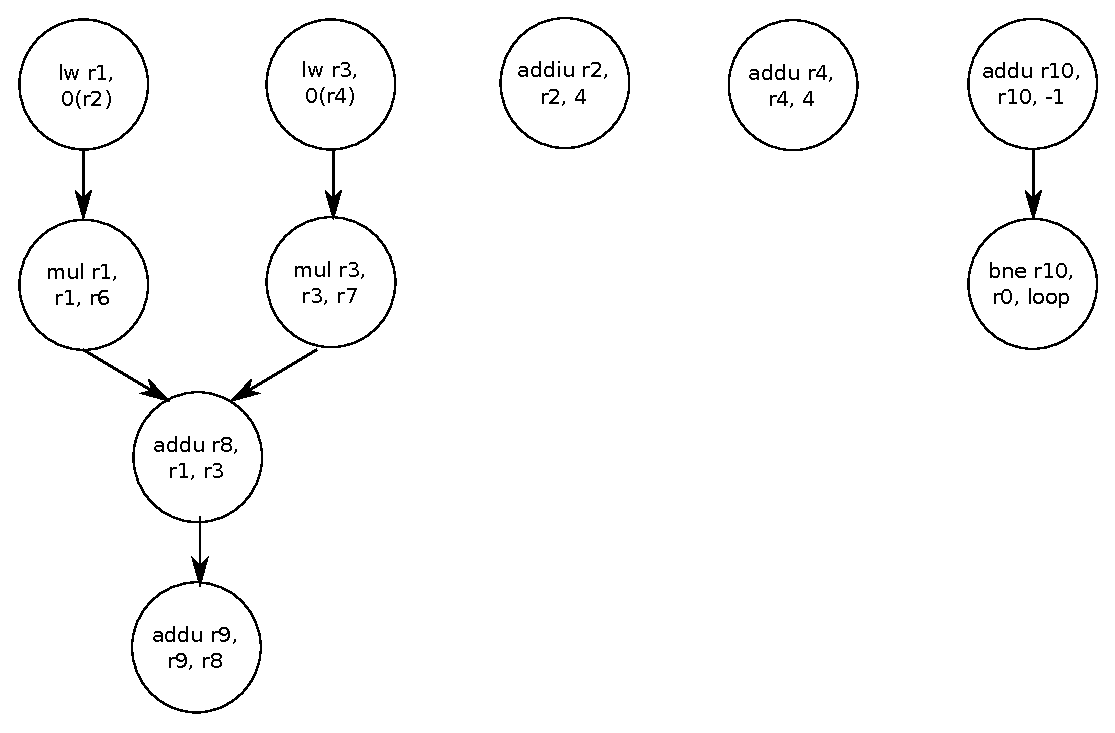
\includegraphics[scale=0.5]{singleiteri.eps}
\label{default}
\end{center}
\caption{Instruction Dependency Graph for Single Iteration}
\end{figure}
The longest path contains 4 nodes.
The ideal ILP for a single iteration is 10/4 = 2.5.

\begin{figure}[H]
\begin{center}
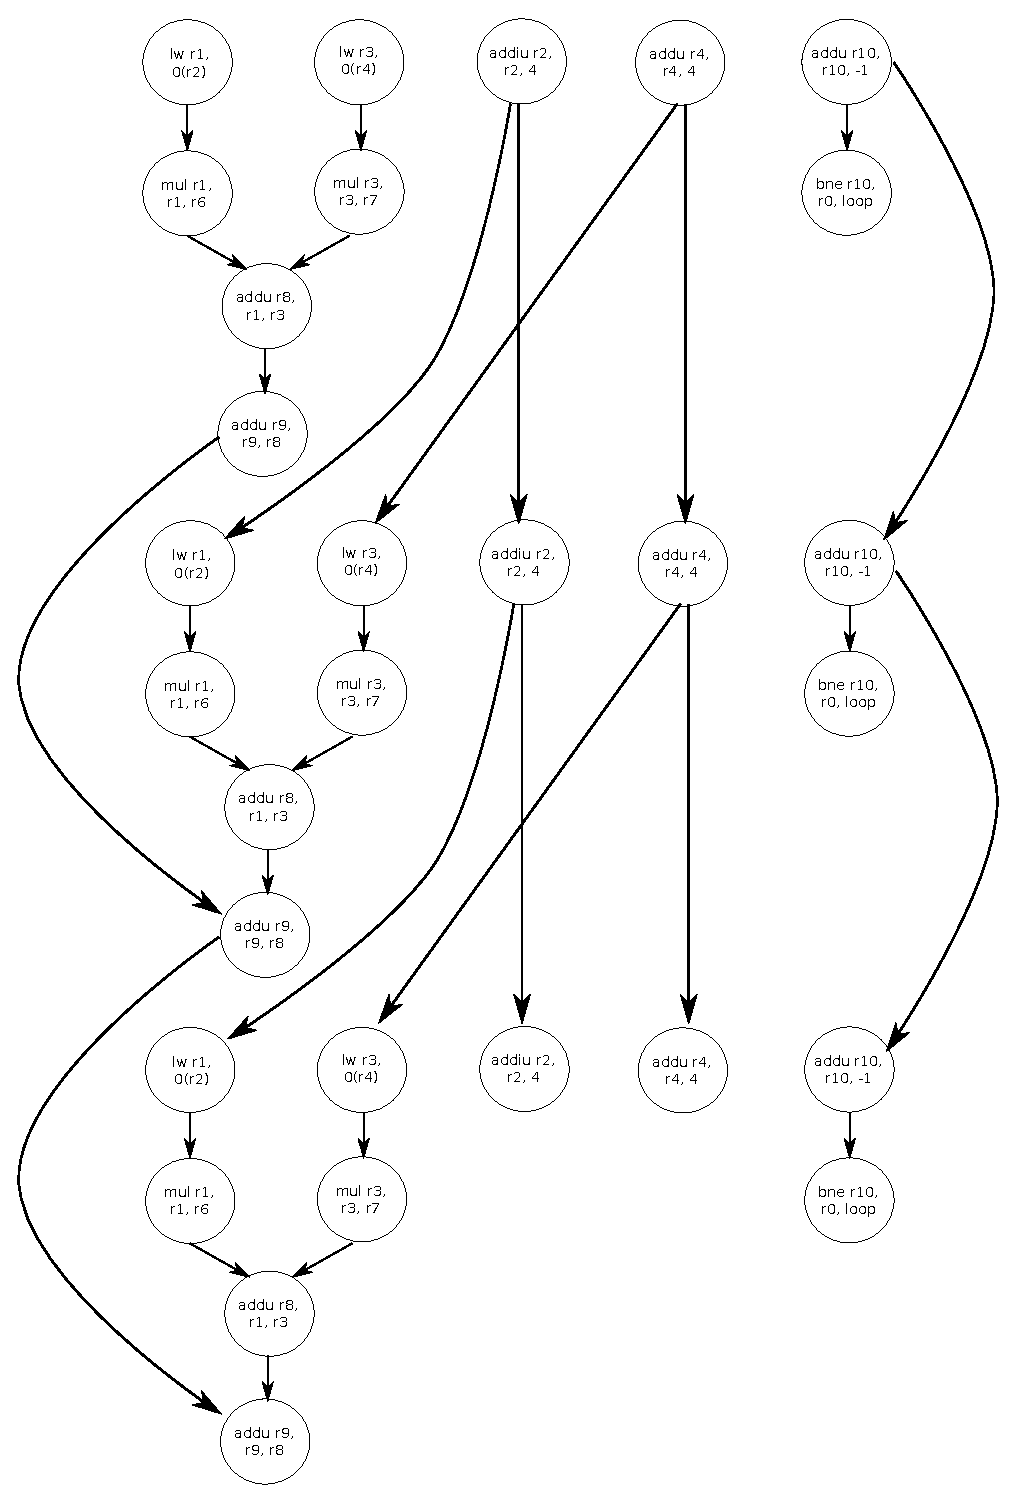
\includegraphics[scale=0.7]{threeiteri.eps}
\label{default}
\end{center}
\caption{Instruction Dependency Graph for Three Iterations}
\end{figure}
The longest path contains 6 nodes. 
The ideal ILP for three iterations is 30/6 = 5.\\

The ideal ILP for N iterations of the loop is simply 10N/(3+N).\\

The IPC of the quad-issue processor is less than the ideal ILP due to several different reasons. The first is that the quad issue processor can only execute at most 4 instructions simultaneously. This thereby limits the IPC to a max of 4. Then, the load word instructions are resolved in the second functional unit in the pipeline, which means that a RAW hazard on the next set of instructions will need to be stalled by 1 cycle. There is also a RAW hazard within a fetch block, so this requires 1 cycle of stalling. Finally, the branch instruction introduces another 2 cycles of delay. There are also 2 squashed instructions in the fetch block with the branch instruction, so this reduced the number of executed instructions for calculating the IPC. In the ideal case, we can execute 12 instructions in 3 cycles, but after adding in the squashed instructions and various delays, we are actually executing 10 instructions in 7 cycles. 

\end{document}